
\chapter{Named Entity Recognition with Incomplete Annotations} % Main chapter title

\label{Chapter5}

In this chapter, we present a practical scenario of named entity recognition. 
We first propose an iterative training approach to this problem and  further discuss the possibility of using dependency tree information to solve this task. 
\section{Introduction}
\label{sec:betterintro}
Named entity recognition (NER) \cite{tjong2002introduction,tjong2003introduction} as one of the most fundamental tasks within natural language processing (NLP) has received significant attention.
%	Most existing approaches to NER focused on a supervised setup, where fully annotated named entity information is assumed to be available during the training phase.
Most existing approaches to NER focused on a supervised setup, where fully annotated named entity information is assumed to be available during the training phase.
%	Most existing approaches to NER focused on a supervised setup, where fully annotated named entity information is assumed to be available during the training phase.
%	The performance of such systems typically depends on the amount and quality of annotated data available.
%	However, in practice, obtaining large-scale high quality annotation can be a very laborious and expensive process.
However, in practice, obtaining high-quality annotations  can be a very laborious and expensive process~\cite{snow2008cheap}. 
One of the common issues with data annotations is there may be incomplete annotations.

%	Most existing approaches to NER focused on a supervised setup, where fully annotated named entity information is assumed to be available during the training phase. The performance of such systems typically depends on the amount and quality of annotated data available. How- ever, in practice, obtaining large-scale high quality annota- tions can be a very laborious and expensive process (Snow et al. 2008). One of the common issues with data annotations is there may be incomplete annotations.

Figure \ref{fig:example1} shows an example sentence with two named entities ``{\em John Lloyd Jones}'' and ``{\em BBC radio}'' of type \textsc{per} (person) and \textsc{org} (organization) respectively. 
Following the standard \textsc{bioes} tagging scheme \cite{ramshaw1999text,ratinov2009design}, the corresponding gold label sequence is shown below the sentence.
When the data annotations are incomplete, certain labels may be missing from the label sequence.
%However, properly defining the task is important, and we argue there are two possible potential pitfalls associated with modeling incomplete annotations, especially for the NER task.
%Specifically, realistic and accurate assumptions need to be made for the {\em available} and {\em unavailable} labels.
%Ensuring both assumptions are valid is crucial for tackling the learning problem with incomplete data annotation.
Properly defining the task is important, and we argue there are two possible potential pitfalls associated with modeling incomplete annotations, especially for the NER task.
\begin{figure}[h!]
	\centering
%	\scalebox{0.68}{
		\begin{tikzpicture}[node distance=1.0mm and 4.0mm, >=Stealth, 
		word/.style={draw=none, minimum height=5mm, rectangle, inner sep=0pt},
		citationbox/.style={draw=puffin, rectangle, minimum height=10mm, minimum width=95mm,line width=1pt, fill=none, text=black,rounded corners=1mm}
		]
		\node [word] (sent) {\it Sentence: };
		\node [word, right= of sent, xshift=-3mm] (chairman) {Chairman};
		\node [word, right= of chairman, color=myred] (john) {\textbf{John}};
		\node [word, right= of john, yshift=-0.5mm, color=myred] (lloyd) {\textbf{Lloyd}};
		\node [word, right= of lloyd, yshift=0.4mm, color=myred] (jones) {\textbf{Jones}};
		\node [word, right= of jones] (said) {said};
		\node [word, right= of said, xshift=-2mm, yshift=-0.4mm] (on) {on};
		\node [word, right= of on, xshift=-1mm, yshift=0.4mm, color=myblue] (bbc) {\textbf{BBC}};
		\node [word, right= of bbc, xshift=1mm, color=myblue] (radio) {\textbf{radio}};
		
		\node[word, below= of sent, yshift=-3mm] (goldo) {\it Gold: };
		\node[word, below= of chairman, yshift=-3mm, color=grass] (l1) {{\textbf{\textsc{o}}}};
		\node[word, below= of john, yshift=-3mm, color=myred] (l2) {{\textbf{\textsc{b}$_{\textsc{per}}$}}};
		\node[word, below= of lloyd, yshift=-2.5mm, color=myred] (l3) {{\textbf{\textsc{i}$_{\textsc{per}}$}}};
		\node[word, below= of jones, yshift=-2.9mm, color=myred] (l4) {{\textbf{\textsc{e}$_{\textsc{per}}$}}};
		\node[word, below= of said, yshift=-3mm, color=grass] (l5) {{\textbf{\textsc{o}}}};
		\node[word, below= of on, yshift=-2.6mm, color=grass] (l6) {{\textbf{\textsc{o}}}};
		\node[word, below= of bbc, yshift=-3.1mm, color=myblue] (l7) {{\textbf{\textsc{b}$_{\textsc{org}}$}}};
		\node[word, below= of radio, yshift=-3.1mm, color=myblue] (l8) {{\textbf{\textsc{e}$_{\textsc{org}}$}}};
		
		\node[word, below= of goldo, yshift=-2mm] (a1) {\it A.1:};
		\node[word, below= of l1, yshift=-2mm, color=grass] (p1) {{\textbf{\textsc{o}}}};
		\node[word, below= of l2, yshift=-2mm, color=myred] (p2) {{\textbf{\textsc{b}$_{\textsc{per}}$}}};
		\node[word, below= of l3, yshift=-2mm, color=mypurple] (p3) {{\textbf{-}}};
		\node[word, below= of l4, yshift=-2mm, color=mypurple] (p4) {\textbf{-}};
		\node[word, below= of l5, yshift=-2mm, color=grass] (p5) {\textbf{\textsc{o}}};
		\node[word, below= of l6, yshift=-2mm, color=mypurple] (p6) {\textbf{-}};
		\node[word, below= of l7, yshift=-2mm, color=mypurple] (p7) {\textbf{-}};
		\node[word, below= of l8, yshift=-2mm, color=myblue] (p8) {\textbf{\textsc{e}$_{\textsc{org}}$}};
		
		\node[word, below right= of p2, yshift=1mm, xshift=-4mm] (c1) {\cite{fernandes2011learning}};
		\node [citationbox, left= of p8, xshift=12mm, yshift=-2mm, text depth=-0.6cm] (c1box) {};
		
		\node[word, below= of a1, yshift=-6mm] (a2) {\it A.2: };
		\node[word, below= of p1, yshift=-6mm, color=grass] (mx1) {\textbf{\textsc{o}}};
		\node[word, below= of p2, yshift=-6mm, color=myred] (mx2) {\textbf{\textsc{b}$_{\textsc{per}}$}};
		\node[word, below= of p3, yshift=-6mm, color=myred] (mx3) {\textbf{\textsc{i}$_{\textsc{per}}$}};
		\node[word, below= of p4, yshift=-6mm, color=myred] (mx4) {\textbf{\textsc{e}$_{\textsc{per}}$}};
		\node[word, below= of p5, yshift=-6mm, color=grass] (mx5) {\textbf{\textsc{o}}};
		\node[word, below= of p6, yshift=-6mm, color=grass] (mx6) {\textbf{\textsc{o}}};
		\node[word, below= of p7, yshift=-6mm, color=mypurple] (mx7) {\textbf{-}};
		\node[word, below= of p8, yshift=-6mm, color=mypurple] (mx8) {\textbf{-}};
		
		\node[word, below right= of mx2, yshift=1mm, xshift=-2mm] (c1) {\cite{carlson2009learning}};
		\node [citationbox, left= of mx8, xshift=7.7mm, yshift=-2mm, text depth=-0.6cm] (c2box) {};
		
		\node[word, below= of a2, yshift=-6mm] (a3) {\it A.3: };
		\node[word, below= of mx1, yshift=-6mm, color=mypurple] (px1) {{\textcolor{mypurple}{-}}};
		\node[word, below= of mx2, yshift=-6mm, color=myred] (px2) {\textbf{\textsc{b}$_{\textsc{per}}$}};
		\node[word, below= of mx3, yshift=-6mm, color=myred] (px3) {\textbf{\textsc{i}$_{\textsc{per}}$}};
		\node[word, below= of mx4, yshift=-6mm, color=myred] (px4) {\textbf{\textsc{e}$_{\textsc{per}}$}};
		\node[word, below= of mx5, yshift=-6mm, color=mypurple] (px5) {\textbf{-}};
		\node[word, below= of mx6, yshift=-6mm, color=mypurple] (px6) {\textbf{-}};
		\node[word, below= of mx7, yshift=-6mm, color=mypurple] (px7) {\textbf{-}};
		\node[word, below= of mx8, yshift=-6mm, color=mypurple] (px8) {\textbf{-}};
		
		\node[word, below right= of px2, yshift=1mm, xshift=7mm] (c3) {Our assumption};
		\node [citationbox, below= of c2box, yshift=-1mm] (c3box) {};
		
		\end{tikzpicture}
%	}
	%	\vspace{-7mm}
	\caption{An example sentence with gold named entity annotations and different assumptions (i.e., \textit{A.1} to \textit{A.3}) on {\em available labels}. ``\textsc{-}'' represents a missing label.}
	%	\vspace{-4.5mm}
	\label{fig:example1}
\end{figure}



Several previous approaches assume the incomplete annotations can be obtained by simply removing either word-level labels \cite{fernandes2011learning} or span-level labels \cite{carlson2009learning}. 
%	As shown in Figure \ref{fig:example1}, both assumptions (i.e., {\it A.1} and {\it A.2}) would result in words annotated with \textsc{o} labels. The former approach may even lead to sub-entity level annotations (e.g., ``{\em radio}'' is annotated as part of an entity).
As shown in Figure \ref{fig:example1}, under both assumptions (i.e., {\it A.1} and {\it A.2}), there will be words annotated with \textsc{o} labels. The former approach may even lead to sub-entity level annotations (e.g., ``{\em radio}'' is annotated as part of an entity).
However, we argue such assumptions can be largely unrealistic.
In practice, annotators are typically instructed to annotate named entities for complete word spans only~\cite{settles2008active,surdeanu2010legal}.
Thus, sub-entity level annotations or \textsc{o} labels \footnote{Why should the \textsc{o} labels be assumed unavailable? This is because  the annotators typically do not actively specify the \textsc{o} labels when working on annotations. If the annotator chooses not to annotate a word, it could either mean it is not part of any entity, {\em or} the word is actually part of an entity but the annotator neglected it in the annotation process (therefore we have incomplete annotations). However, we note that assigning the \textsc{o} label to a word would precisely indicate it is strictly {\em not} part of any entity, which is not desirable.} should not be assumed to be available ({\it A.3}).
Therefore such approaches are making sub-optimal assumptions on the {\em available labels}.





%\citet{fernandes2011learning} assume the incomplete annotations can be obtained by simply discarding some labels from the original gold label sequence.
%As we can see, such an approach may lead to incomplete entities such as ``{\em radio}''. We believe this is not a very realistic setup as in practice the annotators do not provide such sub-entity level annotations.
%\citet{carlson2009learning} approached this problem based on an alternative setup where the labels associated with certain complete entities are missing but \textsc{o} labels are still available.
%However, we note that in practice annotators are typically instructed to annotate entity spans only, ignoring a significant amount of other words in the text. 
%Thus, assuming the availability of \textsc{o} labels that indicate non-entities may be unrealistic as the annotators will not be actively assigning such labels to words.
%As we can see both approaches have limitations associated with their assumptions on the {\em annotated labels}.

When the proper assumptions on the available labels are made, one can typically model the missing labels as latent variables and train a latent-variable conditional random fields model \cite{quattoni2005conditional}.
One such approach is presented in \cite{bellare2007learning}.
Their work focused on the citation parsing\footnote{The task is to tag the BibTex records with different labels (i.e., ``title'', ``author'', ``affiliation'' and so on).} (i.e., sequence labeling) task which does not suffer from the above issue as no \textsc{o} label is involved.
However, though the approach was shown effective in the citation parsing task, we found its effectiveness does not transfer to the NER task even in the absence of the above {available labels} issue.
As we would highlight later, the reason is related to the undesirable assumptions on the {\em unavailable labels}.
%Our further investigations lead to the important notion of {\em latent label distribution} for unlabeled words, to which we provide more details in Section \ref{sec:problem}.
%\citet{bellare2007learning} presented a more realistic setup where the only labels available are those assigned to the entities, as also illustrated in Figure \ref{fig:example1}. They proposed to use a latent-variable conditional random fields (CRF)  model \cite{lafferty2001conditional} to learn the underlying distributions of unavailable labels in the sentence.
%However, while their approach was shown to be effective in the citation parsing task, we found their approach in practice does not work well in the context of NER.
%Our investigations show that this issue is mainly attributed to their assumptions made on the {\em unavailable labels}.
%We tackle this issue by defining the {\em latent label distribution} in Section \ref{luwei:provide section name}.

%In this work, we investigate the issue and highlight the importance of correctly specifying the {\em latent label distribution}, which is especially crucial for the task of NER due to the special nature of such a task.
%We show that the partial CRF approach in fact exploits a simple uniform distribution as their latent label distribution for such a task, whereas our approach is able to provide a more sensible estimation for the latent label distribution.
%, and can lead to significantly better results.

%There are already several approaches that tackle the incomplete data annotation problem. The work of \cite{} presented 
%One of the first questions is what is the more realistic scenario associated with modeling the incomplete annotation. - previous approaches are wrong.

%There are existing approaches that address the incomplete data annotation issue. 
%One notable approach is the the partial CRF model of \cite{bellare2007learning,carlson2009learning}.
%The model is a general approach designed for sequence labeling where the assumption is there are missing labels.
%The true underlying labels are then regarded as latent variables in the training phase. 
%The resulting model is essentially a latent variable CRF -- an approach that has been used in various other applications such as syntactic parsing \cite{petrov-klein:2008:EMNLP}, semantic parsing \cite{Zettlemoyer:2005:LMS:3020336.3020416} and statistical machine translation \cite{blunsom2008discriminative}.

%While such an approach yields reasonable results, we note that the task of named entity recognition has certain special characteristics that distinguish it from many other sequence labeling problems such as Chinese word segmentation and part-of-speech tagging.
%One key observation that we make here is that the named entity recognition task is essentially an {\em unbalanced labeling} problem while many other tasks involve {\em balanced labeling} problem.
%The difference between the two types of problems is, when we cast the problem of named entity recognition as a sequence labeling problem, the annotators typically actively mark the boundaries of entities, assuming the remaining words are assigned the default label \textsc{o} (indicating the word is outside of any entity).

%We call the former  {\em balanced labeling} problem and the latter {\em unbalanced labeling} problem.
%Unfortunately, existing approaches largely focused on the former setup and largely ignored the second setup.
%However, we note that the second setup is more natural and realistic.
%This is because in the annotation process, the annotator typically only actively search for relevant entities and ignore the irrelevant text.
%If a certain text span is ignored, it is usually regarded as irrelevant text and are therefore labeled as \text{o}.
%However, in the event of missing annotations, if a certain text span is not assigned any annotation, there are essentially two possibilities: whether it is o or it is part of an entity but is neglected by the annotator.
%However, in the common setup used in partial CRF, the assumption was many tags are not available. We believe this is not a very realistic setup as in practice the annotators do not actively specify the o tags.
%We present a more realistic setup in practice. 

%In the sequence labeling tasks, we need to predict a label for each token in the input sequence. 
%Partial data annotation in sequence labeling often refers to the missing label information for some tokens in the sequence. 
%Figure \ref{fig:example1} shows an example of two input sequences and each with three corresponding label sequences: POS tags, named entities and sentiment labels. 
%Labels that colored in red are the annotations observed and those colored in blue are not observed under the partial data annotation setting. 
%In this case, we only have the knowledge that ``\textit{Steve}'' is a ``\textsc{Person}'' (\textsc{Per}) entity during the training phase in the NER task. 
%Similar in the second sentence, we can only observe the ``\textit{kimchi}'' is an ``\textsc{Misc}'' entity. 
%The named entity and sentiment label sequences are dominated by the label \textsc{O} (i.e., non-entity) while the POS tag sequence is dominated by any labels. 
%Based on this observation, we categorize sequences like named entities and sentiment labels as ``\textit{unbalanced label sequences}'' and sequences like POS tags as ``\textit{balanced label sequences}''. 
%The label sequences in other tasks such as chunking and Chinese word segmentation~\cite{sun2011enhancing} also refer as ``\textit{balanced label sequences}''. 
%Previous work has shown promising performance on balanced label sequences, such as POS tagging with partial data annotations especially in low-resource language~\cite{tsuboi-EtAl:2008:PAPERS,garrette2012type,garrette2013real,garrette2013learning} and Chinese word segmentation with partially labeled data~\cite{yang2014semi,liu-EtAl:2014:EMNLP2014}. 
%
%In this work, we specifically focus on partial data annotations on the ``\textit{unbalanced label sequence}'' that is present in the task of named entity recognition. 
%Previous work~\cite{carlson2009learning,fernandes2011learning} solved the problem with partial annotations under a setup where the token labels are randomly removed. 
%Unlike previous work, we focus on a more challenging and realistic setup where the information of the dominated label (i.e., \textsc{O} label in our case) is always unknown and the entity (or targeted sentiment) labels are randomly removed. 
%In practice, annotators are often asked to annotate what are the specific entities based on specific requirements. 
%For example, annotators can be asked to annotate the entities with ``\textit{brand}'' while there are still ``\textit{material}'' entities in the sentences. 
%Under this challenging setup, we analyze and empirically show the difficulties for traditional models such as partial conditional random fields (CRF). 
%They might suffer from unbalanced label issue when we have no \textsc{O} type annotations at all. 
%The annotations for \textsc{O} types and other entity labels are all unknown though most of the tokens should be labeled as \textsc{O}. 
%Common sequence labeling models such as conditional random fields (CRF) probably try to predict most of the tokens as entities as we do not have any \textsc{O} type annotations in the training data at all. 
%Inspired by \newcite{dredze2009sequence}, we then propose our bootstrapping CRF model to attack the difficulties by splitting the datasets into multiple parts and applying estimation distribution on the unlabeled tokens. 
%The estimation distribution is trained on some parts of the dataset and then applied on the other part of the dataset. 

In this work, we tackle the incomplete annotation problem when building an NER system, under a more realistic yet more challenging scenario. 
We present a novel, effective, yet easy-to-implement approach, and conduct extensive experiments on various datasets and show our approach significantly outperforms several previous approaches.

%In this work, we resolve both of the above issues and propose a better approach for modeling incomplete annotation for the task of named entity recognition.
%Specifically, we make the following major contributions:
%\squishlist
%\item We tackle the incomplete annotation problem under a challenging yet more realistic scenario for learning named entity recognition systems.
%% from incomplete annotation.
%%\item We present the difficulties of a challenging partial data annotation problem for traditional models. 
%\item We present a novel, effective, yet easy-to-implement approach for NER with incomplete data annotation based on our practical setup.
%%\item We propose a self-learning model for sequence labeling with partial data annotation. The proposed approach makes use of the advantages of multiple parts of datasets and performs self training to improve the performance. 
%\item We conduct extensive experiments on various datasets and show our approach \footnote{Our code will be made available for download.} significantly outperforms several previous approaches.

%\item Extensive experiments conducted on the five datasets prove the effectiveness of the proposed approach\footnote{Our code will be released under *URL*}. 
%\squishend


\section{Related Work}
Previous research efforts on partially annotated data are mostly based on the conditional random fields (CRF)~\cite{lafferty2001conditional}, structured perceptron~\cite{collins2002discriminative} and max-margin~\cite{tsochantaridis2005large} (e.g. structural support vector machine) models.
%	 (i.e., structured perceptron and support vector machines). 
\citet{bellare2007learning} proposed a missing label linear-chain CRF\footnote{This model was also named as Partial CRF~\cite{carlson2009learning} and EM Marginal CRF~\cite{greenberg2018marginal}.} which is essentially a latent-variable CRF~\cite{quattoni2005conditional} on citation parsing~\cite{mccallum2000automating}.
This model had also been used in part-of-speeching tagging and segmentation task with incomplete annotations~\cite{tsuboi-EtAl:2008:PAPERS, liu-EtAl:2014:EMNLP2014,yang2014semi}. 
\citet{yang2018distantly} showed the effectiveness of such a model on Chinese NER with incomplete annotations due to the fact that they required a certain number of fully annotated data to perform joint training. 
\citet{greenberg2018marginal} applied this model on a biomedical NER task and achieved promising performance with incomplete annotations. 
However, in their assumption for the incomplete annotations, the \textsc{O} labels are still considered, which we believe is not realistic. 
%	achieved promising performance on the biomedical NER task with this model but {\color{red}their assumption largely reduces the number of {\it unavailable labels}}. 
\citet{carlson2009learning} modified the structured perceptron algorithm and defined features only on the tokens with annotated labels in partially labeled sequences. 
\citet{fernandes2011learning} and \citet{lou2012structured} proposed to use a large-margin learning framework similar to structured support vector machines with latent variables~\cite{yu2009learning}. 




\section{Approach}
\label{sec:problem}

Given the input word sequence $\vec{x}$, the NER task is to predict a label sequence $\vec{y}$ that encodes the NER information (e.g., in a form following the \textsc{bioes} tagging scheme). Given a training set that consists of completely labeled data $\mathcal{D}$, one can tackle this problem using a standard linear-chain conditional random field (CRF) \cite{lafferty2001conditional} whose loss function is as follows:\footnote{In practice, we also have an $L_2$ regularization term, which we exclude from the formula for brevity.}
\begin{equation}
\mathcal{L}(\vec{w}) 
=
-
\sum_{i}
\log
p_{\vec{w}} (\vec{y}^{(i)} \vert \vec{x}^{(i)}) 
\end{equation}
%	\begin{center}
%		\begin{tabular}{c}
%			$
%				\mathcal{L}(\vec{w}) 
%			=
%			-
%			\sum_{i}
%			\log
%			p_{\vec{w}} (\vec{y}^{(i)} \vert \vec{x}^{(i)}) 
%			$
%		\end{tabular}
%		%\vspace{-2mm}
%	\end{center}
where $(\mathbf{x}^{(i)}, \mathbf{y}^{(i)})$ is the $i$-th instance from $\mathcal{D}$. 
%	, $\kappa$ is the $\ell_2$ coefficient and $\mathbf{w}$  the model parameters.
%$p_{\mathbf{w}}(\mathbf{y}|\mathbf{x})$ can be parameterized as:
%\begin{align}
%p_\vec{w} (\vec{y}|\vec{x}) 
%= \frac{\exp(\vec{w}\cdot\vec{f}(\vec{x}, \vec{y}))}{\sum_{\vec{y}'} \exp(\vec{w}\cdot\vec{f}(\vec{x}, \vec{y}'))} 
%\end{align}

%We can also rewrite the above function as:
%% in the following form:
%\begin{align}
%%\mathcal{L}(\vec{w}) 
%%=& 
%-\sum_{i}
%\log
%\sum_{ \vec{y} } 
%q_{\mathcal{D}} (\vec{y} | \vec{x}^{(i)}) 
%p_{\vec{w}} (\vec{y} \vert \vec{x}^{(i)}) 
%%\nonumber\\
%%&
%\label{equ:finalobj2}
%\end{align}
%where $q_{\mathcal{D}} (\vec{y} | \vec{x}^{(i)})$ will be an indicator function that returns 1 if and only if $\mathbf{y}=\mathbf{y}^{(i)}$.
%Note that in the above function $\mathbf{y}$ or $\mathbf{y}^{(i)}$ are assumed to be complete label sequences. 

%%%%%%%% BEGIN OF 4 FIGURES %%%%%%%

%%%%%%%% BEGIN OF 4 FIGURES %%%%%%%
\begin{figure*}[h!]
	%		\centering
	\begin{subfigure}{0.5\textwidth}
		\centering
		\scalebox{0.5}{
			\begin{tikzpicture}[node distance=2.0mm and 6.0mm, >=Stealth, 
			word/.style={draw=none, minimum height=5mm, rectangle},
			olabel/.style={draw=none, circle, minimum height=9mm, minimum width=9mm,line width=1pt, inner sep=2pt, fill=grass, text=fontgray, label={center:\textbf{\textsc{o}}}, fill opacity=0.5},
			bperlabel/.style={draw=none, circle, minimum height=9mm, minimum width=9mm,line width=1pt, inner sep=2pt, fill=myred, text=black, label={center:\textbf{\textsc{per}}}, fill opacity=0.7},
			borglabel/.style={draw=none, circle, minimum height=9mm, minimum width=9mm,line width=1pt, inner sep=2pt, fill=lowblue, text=black, label={center:\textbf{\textsc{org}}}, fill opacity=0.8},
			invis/.style={draw=none, circle, minimum height=9mm, minimum width=9mm,line width=1pt, inner sep=2pt, fill=none, text=fontgray},
			chainLine/.style={line width=1pt,-, color=fontgray}	%		,background rectangle/.style={fill=olive!45}, show background rectangle
			]
			\node[word](p0) [] {\it Chairman};
			\node[word](p1) [right = of p0] {\it John};
			\node[word](p2) [right = of p1] {\it Lloyd};
			\node[word](p3) [right = of p2] {\it Jones};
			\node[word](p4) [right = of p3] {\it said};
			\node[word, xshift=3mm](p5) [right = of p4] {\it on};
			\node[word, xshift=1.5mm](p6) [right = of p5] {\it BBC};
			\node[word](p7) [right = of p6] {\it radio};
			\node[olabel](t0o) [below = of p0, yshift=2mm] {};
			\node[invis](t0bper) [below = of t0o] {};
			%			\node[word](graphlabel) [left = of t0bper, xshift=-2mm] {\Large (a) {\it Gold}};
			
			\node[invis](t1o) [below = of p1, yshift=2mm] {};
			\node[bperlabel](t1per) [below = of t1o] {};
			
			\node[invis](t2o) [below = of p2, yshift=2mm] {};
			\node[bperlabel](t2per) [below = of t2o] {};
			
			\node[invis](t3o) [below = of p3, yshift=2mm] {};
			\node[bperlabel](t3per) [below = of t3o] {};
			
			\node[olabel](t4o) [below = of p4, yshift=2mm] {};
			
			\node[olabel](t5o) [below = of p5, yshift=2mm] {};
			
			\node[invis](t6o) [below = of p6, yshift=2mm] {};
			\node[invis](t6per) [below = of t6o] {};
			\node[borglabel](t6org) [below = of t6per] {};
			
			\node[invis](t7o) [below = of p7, yshift=2mm] {};
			\node[invis](t7per) [below = of t7o] {};
			\node[borglabel](t7org) [below = of t7per] {};
			
			
			\begin{pgfonlayer}{background}
			\draw [chainLine] (t0o) to (t1per);
			\draw [chainLine] (t1per) to (t2per);
			\draw [chainLine] (t2per) to (t3per);
			\draw [chainLine] (t3per) to (t4o);
			\draw [chainLine] (t4o) to (t5o);
			\draw [chainLine] (t5o) to (t6org);
			\draw [chainLine] (t6org) to (t7org);
			\end{pgfonlayer}
			
			
			
			\end{tikzpicture}
		}
		%			\vspace{-4mm}
		%			\caption{\em Gold}
		\label{fig:groundtruth}
		\caption{\textit{Gold}}
	\end{subfigure}
	\begin{subfigure}{0.5\textwidth}
		\centering
		\scalebox{0.5}{
			\begin{tikzpicture}[node distance=2.0mm and 6.0mm, >=Stealth, 
			word/.style={draw=none, minimum height=5mm, rectangle},
			olabel/.style={draw=none, circle, minimum height=9mm, minimum width=9mm,line width=1pt, inner sep=2pt, fill=grass, text=fontgray, label={center:\textbf{\textsc{o}}}, fill opacity=0.5},
			bperlabel/.style={draw=none, circle, minimum height=9mm, minimum width=9mm,line width=1pt, inner sep=2pt, fill=myred, text=black, label={center:\textbf{\textsc{per}}}, fill opacity=0.7},
			borglabel/.style={draw=none, circle, minimum height=9mm, minimum width=9mm,line width=1pt, inner sep=2pt, fill=lowblue, text=black, label={center:\textbf{\textsc{org}}}, fill opacity=0.8},
			invis/.style={draw=none, circle, minimum height=9mm, minimum width=9mm,line width=1pt, inner sep=2pt, fill=none, text=fontgray},
			chainLine/.style={line width=1pt,-, color=fontgray}	%		,background rectangle/.style={fill=olive!45}, show background rectangle
			]
			\node[word](p0) [] {\it Chairman};
			\node[word](p1) [right = of p0] {\it John};
			\node[word](p2) [right = of p1] {\it Lloyd};
			\node[word](p3) [right = of p2] {\it Jones};
			\node[word](p4) [right = of p3] {\it said};
			\node[word, xshift=3mm](p5) [right = of p4] {\it on};
			\node[word, xshift=1.5mm](p6) [right = of p5] {\it BBC};
			\node[word](p7) [right = of p6] {\it radio};
			\node[olabel](t0o) [below = of p0, yshift=2mm] {};
			\node[invis](t0bper) [below = of t0o, yshift=2mm] {};
			%			\node[word](graphlabel) [left = of t0bper, xshift=3mm] {\Large (b) {\it Simple}};
			
			\node[invis](t1o) [below = of p1, yshift=2mm] {};
			\node[bperlabel](t1per) [below = of t1o] {};
			
			\node[invis](t2o) [below = of p2, yshift=2mm] {};
			\node[bperlabel](t2per) [below = of t2o] {};
			
			\node[invis](t3o) [below = of p3, yshift=2mm] {};
			\node[bperlabel](t3per) [below = of t3o] {};
			
			\node[olabel](t4o) [below = of p4, yshift=2mm] {};
			
			\node[olabel](t5o) [below = of p5, yshift=2mm] {};
			
			\node[olabel](t6o) [below = of p6, yshift=2mm] {};
			\node[invis](t6per) [below = of t6o] {};
			\node[invis](t6org) [below = of t6per] {};
			
			\node[olabel](t7o) [below = of p7, yshift=2mm] {};
			\node[invis](t7per) [below = of t7o] {};
			\node[invis](t7org) [below = of t7per] {};
			
			\begin{pgfonlayer}{background}
			\draw [chainLine] (t0o) to (t1per);
			\draw [chainLine] (t1per) to (t2per);
			\draw [chainLine] (t2per) to (t3per);
			\draw [chainLine] (t3per) to (t4o);
			\draw [chainLine] (t4o) to (t5o);
			\draw [chainLine] (t5o) to (t6o);
			\draw [chainLine] (t6o) to (t7o);
			
			
			\end{pgfonlayer}
			\end{tikzpicture}
		}
		%		\vspace{-4mm}
		%			\caption{\textit{Simple}}
		%			\vspace{-1mm}
		\caption{\textit{Simple}}
	\end{subfigure}
	%	\vspace{-5mm}
\end{figure*}
\begin{figure*}[h!]
	\begin{subfigure}{0.5\textwidth}
		\centering
		\scalebox{0.5}{
			\begin{tikzpicture}[node distance=2.0mm and 6.0mm, >=Stealth, 
			word/.style={draw=none, minimum height=5mm, rectangle},
			olabel/.style={draw=none, circle, minimum height=9mm, minimum width=9mm,line width=1pt, inner sep=2pt, fill=grass, text=fontgray, label={center:\textbf{\textsc{o}}}, fill opacity=0.5},
			bperlabel/.style={draw=none, circle, minimum height=9mm, minimum width=9mm,line width=1pt, inner sep=2pt, fill=myred, text=black, label={center:\textbf{\textsc{per}}}, fill opacity=0.7},
			borglabel/.style={draw=none, circle, minimum height=9mm, minimum width=9mm,line width=1pt, inner sep=2pt, fill=lowblue, text=black, label={center:\textbf{\textsc{org}}}, fill opacity=0.8},
			invis/.style={draw=none, circle, minimum height=9mm, minimum width=9mm,line width=1pt, inner sep=2pt, fill=none, text=fontgray},
			chainLine/.style={line width=1pt,-, color=fontgray}	%		,background rectangle/.style={fill=olive!45}, show background rectangle
			]
			\node[word](p0) [] {\it Chairman};
			\node[word](p1) [right = of p0] {\it John};
			\node[word](p2) [right = of p1] {\it Lloyd};
			\node[word](p3) [right = of p2] {\it Jones};
			\node[word](p4) [right = of p3] {\it said};
			\node[word, xshift=3mm](p5) [right = of p4] {\it on};
			\node[word, xshift=1.5mm](p6) [right = of p5] {\it BBC};
			\node[word](p7) [right = of p6] {\it radio};
			
			\node[olabel](t0o) [below = of p0, yshift=2mm] {};
			\node[bperlabel](t0per) [below = of t0o] {};
			\node[borglabel](t0org) [below = of t0per] {};
			
			%			\node[word](graphlabel) [left = of t0bper, xshift=5mm] {\Large (c) {\it Uniform}};
			
			\node[invis](t1o) [below = of p1, yshift=2mm] {};
			\node[bperlabel](t1per) [below = of t1o] {};
			
			\node[invis](t2o) [below = of p2, yshift=2mm] {};
			\node[bperlabel](t2per) [below = of t2o] {};
			
			\node[invis](t3o) [below = of p3, yshift=2mm] {};
			\node[bperlabel](t3per) [below = of t3o] {};
			
			\node[olabel](t4o) [below = of p4, yshift=2mm] {};
			\node[bperlabel](t4per) [below = of t4o] {};
			\node[borglabel](t4org) [below = of t4per] {};
			
			\node[olabel](t5o) [below = of p5, yshift=2mm] {};
			\node[bperlabel](t5per) [below = of t5o] {};
			\node[borglabel](t5org) [below = of t5per] {};
			
			\node[olabel](t6o) [below = of p6, yshift=2mm] {};
			\node[bperlabel](t6per) [below = of t6o] {};
			\node[borglabel](t6org) [below = of t6per] {};
			
			\node[olabel](t7o) [below = of p7, yshift=2mm] {};
			\node[bperlabel](t7per) [below = of t7o] {};
			\node[borglabel](t7org) [below = of t7per] {};
			
			
			\begin{pgfonlayer}{background}
			
			\draw [chainLine] (t0o) to (t1per);
			\draw [chainLine] (t0per) to (t1per);
			\draw [chainLine] (t0org) to (t1per);
			
			\draw [chainLine] (t1per) to (t2per);
			\draw [chainLine] (t2per) to (t3per);
			
			\draw [chainLine] (t3per) to (t4o);
			\draw [chainLine] (t3per) to (t4per);
			\draw [chainLine] (t3per) to (t4org);
			
			\draw [chainLine] (t4o) to (t5o);
			\draw [chainLine] (t4o) to (t5per);
			\draw [chainLine] (t4o) to (t5org);
			\draw [chainLine] (t4per) to (t5o);
			\draw [chainLine] (t4per) to (t5per);
			\draw [chainLine] (t4per) to (t5org);
			\draw [chainLine] (t4org) to (t5o);
			\draw [chainLine] (t4org) to (t5per);
			\draw [chainLine] (t4org) to (t5org);
			
			\draw [chainLine] (t5o) to (t6o);
			\draw [chainLine] (t5o) to (t6per);
			\draw [chainLine] (t5o) to (t6org);
			\draw [chainLine] (t5per) to (t6o);
			\draw [chainLine] (t5per) to (t6per);
			\draw [chainLine] (t5per) to (t6org);
			\draw [chainLine] (t5org) to (t6o);
			\draw [chainLine] (t5org) to (t6per);
			\draw [chainLine] (t5org) to (t6org);
			
			\draw [chainLine] (t6o) to (t7o);
			\draw [chainLine] (t6o) to (t7per);
			\draw [chainLine] (t6o) to (t7org);
			\draw [chainLine] (t6per) to (t7o);
			\draw [chainLine] (t6per) to (t7per);
			\draw [chainLine] (t6per) to (t7org);
			\draw [chainLine] (t6org) to (t7o);
			\draw [chainLine] (t6org) to (t7per);
			\draw [chainLine] (t6org) to (t7org);
			
			
			\end{pgfonlayer}
			
			
			
			\end{tikzpicture}
		}
		%			\vspace{-2mm}
		%			\caption{\em Uniform}
		\caption{\textit{Uniform}}
		\label{fig:unifrom}
	\end{subfigure}
	\begin{subfigure}{0.5\textwidth}
		\centering
		\scalebox{0.5}{
			\begin{tikzpicture}[node distance=2.0mm and 6.0mm, >=Stealth, 
			word/.style={draw=none, minimum height=5mm, rectangle},
			olabel/.style={draw=none, circle, minimum height=9mm, minimum width=9mm,line width=1pt, inner sep=2pt, fill=grass, text=fontgray, label={center:\textbf{\textsc{o}}}, fill opacity=0.5},
			bperlabel/.style={draw=none, circle, minimum height=9mm, minimum width=9mm,line width=1pt, inner sep=2pt, fill=myred, text=black, label={center:\textbf{\textsc{per}}}, fill opacity=0.7},
			borglabel/.style={draw=none, circle, minimum height=9mm, minimum width=9mm,line width=1pt, inner sep=2pt, fill=lowblue, text=black, label={center:\textbf{\textsc{org}}}, fill opacity=0.8},
			invis/.style={draw=none, circle, minimum height=9mm, minimum width=9mm,line width=1pt, inner sep=2pt, fill=none, text=fontgray},
			chainLine/.style={line width=1pt,-, color=fontgray}	%		,background rectangle/.style={fill=olive!45}, show background rectangle
			]
			\node[word](p0) [] {\it Chairman};
			\node[word](p1) [right = of p0] {\it John};
			\node[word](p2) [right = of p1] {\it Lloyd};
			\node[word](p3) [right = of p2] {\it Jones};
			\node[word](p4) [right = of p3] {\it said};
			\node[word, xshift=3mm](p5) [right = of p4] {\it on};
			\node[word, xshift=1.5mm](p6) [right = of p5] {\it BBC};
			\node[word](p7) [right = of p6] {\it radio};
			
			\node[olabel](t0o) [below = of p0, yshift=2mm] {};
			\node[bperlabel, fill opacity=0.2](t0per) [below = of t0o] {};
			\node[borglabel, fill opacity=0.2](t0org) [below = of t0per] {};
			%			\node[word](graphlabel) [left = of t0bper, xshift=-1mm] {\Large (d) {\it Ours}};
			
			\node[invis](t1o) [below = of p1, yshift=2mm] {};
			\node[bperlabel](t1per) [below = of t1o] {};
			
			\node[invis](t2o) [below = of p2, yshift=2mm] {};
			\node[bperlabel](t2per) [below = of t2o] {};
			
			\node[invis](t3o) [below = of p3, yshift=2mm] {};
			\node[bperlabel](t3per) [below = of t3o] {};
			
			\node[olabel](t4o) [below = of p4, yshift=2mm] {};
			\node[bperlabel, fill opacity=0.2](t4per) [below = of t4o] {};
			\node[borglabel, fill opacity=0.2](t4org) [below = of t4per] {};
			
			\node[olabel](t5o) [below = of p5, yshift=2mm] {};
			\node[bperlabel, fill opacity=0.2](t5per) [below = of t5o] {};
			\node[borglabel, fill opacity=0.2](t5org) [below = of t5per] {};
			
			\node[olabel, fill opacity=0.2](t6o) [below = of p6, yshift=2mm] {};
			\node[bperlabel, fill opacity=0.2](t6per) [below = of t6o] {};
			\node[borglabel](t6org) [below = of t6per] {};
			
			\node[olabel, fill opacity=0.2](t7o) [below = of p7, yshift=2mm] {};
			\node[bperlabel, fill opacity=0.2](t7per) [below = of t7o] {};
			\node[borglabel](t7org) [below = of t7per] {};
			
			\begin{pgfonlayer}{background}
			\draw [chainLine] (t0o) to (t1per);
			\draw [chainLine] (t0per) to (t1per);
			\draw [chainLine] (t0org) to (t1per);
			
			\draw [chainLine] (t1per) to (t2per);
			\draw [chainLine] (t2per) to (t3per);
			
			\draw [chainLine] (t3per) to (t4o);
			\draw [chainLine] (t3per) to (t4per);
			\draw [chainLine] (t3per) to (t4org);
			
			\draw [chainLine] (t4o) to (t5o);
			\draw [chainLine] (t4o) to (t5per);
			\draw [chainLine] (t4o) to (t5org);
			\draw [chainLine] (t4per) to (t5o);
			\draw [chainLine] (t4per) to (t5per);
			\draw [chainLine] (t4per) to (t5org);
			\draw [chainLine] (t4org) to (t5o);
			\draw [chainLine] (t4org) to (t5per);
			\draw [chainLine] (t4org) to (t5org);
			
			\draw [chainLine] (t5o) to (t6o);
			\draw [chainLine] (t5o) to (t6per);
			\draw [chainLine] (t5o) to (t6org);
			\draw [chainLine] (t5per) to (t6o);
			\draw [chainLine] (t5per) to (t6per);
			\draw [chainLine] (t5per) to (t6org);
			\draw [chainLine] (t5org) to (t6o);
			\draw [chainLine] (t5org) to (t6per);
			\draw [chainLine] (t5org) to (t6org);
			
			\draw [chainLine] (t6o) to (t7o);
			\draw [chainLine] (t6o) to (t7per);
			\draw [chainLine] (t6o) to (t7org);
			\draw [chainLine] (t6per) to (t7o);
			\draw [chainLine] (t6per) to (t7per);
			\draw [chainLine] (t6per) to (t7org);
			\draw [chainLine] (t6org) to (t7o);
			\draw [chainLine] (t6org) to (t7per);
			\draw [chainLine] (t6org) to (t7org);
			
			
			\end{pgfonlayer}
			
			\end{tikzpicture}
		}
		%			\vspace{-1mm}
		%			\caption{\em Ours}
		\caption{\textit{Ours}}
		\label{fig:ours}
	\end{subfigure}
	
	%		\vspace{-2mm}
	\caption{Graphical illustrations on different assumptions on {\em unavailable labels}, where the entity ``{\em John Lloyd Jones}'' of type \textsc{per} is labeled but ``{\em BBC radio}'' of type \textsc{org} is missing. Each path refers to one possible complete label sequence, and the density of the color indicates probability (we excluded \textsc{b} and \textsc{e} tags for brevity).}
	%		\vspace{-4mm}
	\label{fig:nerlabelseq}
\end{figure*}
%%%%%%%% END OF 4 FIGURES %%%%%%%
%%%%%%%% END OF 4 FIGURES %%%%%%%


Now, assume we have an incomplete label sequence $\mathbf{y}_p^{(i)}$. From such a $\mathbf{y}_p^{(i)}$ we should be able to derive a set of all possible complete label sequences that are compatible with (i.e., contain) the incomplete label sequence, and let us call this set $\mathcal{C}(\mathbf{y}_p^{(i)})$. 
%	Apparently, $\mathcal{C}(\mathbf{y}^{(i)})=\{\mathbf{y}^{(i)}\}$ for a complete label sequence $\mathbf{y}^{(i)}$. 
We can  rewrite the above function as:
%	\begin{center}
%		\begin{tabular}{c}
%			$
%			\mathcal{L}(\vec{w}) 
%			= 
%			-
%%			\!\!
%			\sum\limits_{i}
%			\log
%%			\!\!\!
%%			\!\!\!\!
%			\sum\limits_{ \vec{y}\in\mathcal{C}(\mathbf{y}^{(i)}_p) } 
%%			\!\!\!\!
%			q_{\mathcal{D}} (\vec{y} | \vec{x}^{(i)}) 
%			p_{\vec{w}} (\vec{y} \vert \vec{x}^{(i)}) 
%			$
%		\end{tabular}
%		%\vspace{-2mm}
%	\end{center}
\begin{align}
\mathcal{L}(\vec{w}) 
=& 
-
\sum_{i}
\log
\sum_{ \vec{y}\in\mathcal{C}(\mathbf{y}^{(i)}_p) } 
q_{\mathcal{D}} (\vec{y} | \vec{x}^{(i)}) 
p_{\vec{w}} (\vec{y} \vert \vec{x}^{(i)}) 
\nonumber
%&
\label{equ:finalobj3}
\end{align}

%	Understanding the loss function from such a perspective helps us establish a unified view of various approaches to learning with incomplete annotation.
%	Based on such a unified view we also develop our own approach.
%It is also helpful for developing our new approach.

We illustrate in Figure \ref{fig:nerlabelseq} several previous approaches as well as our approach. 
In this example, the entity {\em BBC radio} of type \textsc{org} is not annotated.
Figure \ref{fig:nerlabelseq}(a) shows a single path that corresponds to the gold label sequence.
Figure \ref{fig:nerlabelseq}(b) illustrates a naive approach, where we regard all the missing labels as \textsc{o} labels. 
This essentially assumes that the $q$ distribution in the above equation puts all probability mass to this single label sequence, which is an incorrect assumption.   
%	Unfortunately as we can see this is an incorrect assumption.

%We will use such a form to develop our approach when we have incomplete data annotation.
%The NER task is a sequence labeling problem, where we would like to predict a label sequence $\vec{y} = \{y_{1}, y_{2}, \cdots, y_{n}\}$ given an observation sequence $\vec{x} = \{x_{1}, x_{2}, \cdots, x_{n}\}$ where $n$ is the number of tokens in the sequence. 
%As the training data is partially annotated, each instance in the training set $\mathcal{D}$ is therefore represented as an ordered pair $(\vec{x}, \vec{y}_p)$ where $\vec{y}_p$ represents a partial label sequence. 
%As we conduct experiments on named entity recognition and targeted sentiment analysis, the label set is named entities and sentiment labels for two tasks, respectively. 
%Additionally, we use the \textsc{o} label to denote tokens that do not belong to entities.
% or sentiment classes.
%those tokens not labeled as entities or sentiment classes.  
%As we have seen in the previous sections, the label sequences both NER and entity-level sentiment analysis tasks are dominated by the $\mathbf{O}$ label. 
%We study the partial data annotation problem under a challenging setup during the training phase: 
%
%\begin{center}
%	\textit{Only a few (complete) entities are observed for each sentence, which means no annotation on $\mathbf{O}$ label is observed.}
%\end{center}
%
%In practice, we usually annotate the entity type information and sometimes only the specific entity type as only those are important for a specific dataset. 
%However, the dataset might contains other entity types which are not annotated but annotated in other datasets. 
%Our setup above indicates this scenario in practice. 
%For example in Figure \ref{fig:example1}, some might be interested in \textsc{per} entities only, thus the annotation only show the positions where we have the \textsc{per}. 



Now let us look at what assumptions on $q$ have been made by the existing approach of~\cite{bellare2007learning}.
The model regards the missing labels as latent variables and learns a latent variable CRF using the following loss:
%	\begin{center}
%		\begin{tabular}{c}
%			$
%				-\sum_{i}
%			\log
%			\sum_{ \vec{y}\in\mathcal{C}(\mathbf{y}^{(i)}_p) } 
%			p_{\vec{w}} (\vec{y} \vert \vec{x}^{(i)}) 
%			$
%		\end{tabular}
%	\end{center}
\begin{align}
-\sum_{i}
\log
\sum_{ \vec{y}\in\mathcal{C}(\mathbf{y}^{(i)}_p) } 
p_{\vec{w}} (\vec{y} \vert \vec{x}^{(i)}) 
%\nonumber\\
%&
\end{align}

The resulting model is called {\em missing label linear-chain CRF} ({\em M-CRF})~\footnote{Similar assumptions have also been made by \cite{carlson2009learning,fernandes2011learning}, but they used structured perceptron \cite{collins2002discriminative} instead.}. As we can see from the above function, this is essentially equivalent to say $q$ is a uniform distribution that assigns equal probabilities to all possible complete label sequences in $\mathcal{C}(\mathbf{y}_p^{(i)})$.

We believe such an assumption on $q$ that describes {\em unavailable labels} can be improved. As we can see from the above example in Figure \ref{fig:nerlabelseq}(d), a more desirable assumption about $q$ is to put more probability mass to a path that is close to the gold path. 
In practice, their approach worked for the task of citation parsing, where the $q$ distribution may not deviate much from the uniform distribution (Figure \ref{fig:nerlabelseq}(c)) in such a task. However, in the task of NER, we find such a simple treatment to the $q$ distribution often leads to sub-optimal results (as we can see in the experiments later) as the $q$ distribution is highly skewed due to the large amount of \textsc{o} labels.
This observation motivates us to find a proper way to define $q$ that can approximate the gold label distribution in this work.


% using conditional random fields~\cite{lafferty2001conditional} and structured perceptron~\cite{collins2002discriminative} performs well by learning from the partially annotated sequences. 
%The intuition is learning from those labeled tokens and helping the model to identify unlabeled tokens. 
%For example, under the assumptions from \cite{bellare2007learning} and \cite{fernandes2011learning} in Figure \ref{fig:example1}, such models can learn ``\textit{John}'' is with label ``\textsc{b}$_\textsc{per}$'' and ``said'' is with label ``\textsc{o}''. 
%In this case, the models are still able to learn to recognize different labels as those labels appear during training. 
%However, under our realistic assumption, we have no gold information about the words associated with \textsc{o} labels. 
%Training such models will lead to a problem of high recall and low precision. 
%The common model to tackle this problem is to introduce a latent variable in conditional random fields~\cite{lafferty2001conditional} model and marginalize over all the possible latent sequences. 
%Let $\mathcal{C}(\vec{y}_p)$ set represents all the possible sequences that contain the partial sequence $\vec{y}_p$. 
%The training objective is to maximize the following marginalized log-likelihood:
%\begin{align}
%%\log \sum_{ \vec{y} \in \mathcal{C}(\vec{y}_p) }
%%\frac{\exp(\vec{w}\cdot\vec{f}(\vec{x}, \vec{y}))}{\sum_{\vec{y}^{'}\in \mathcal{Y}} \exp(\vec{w}\cdot\vec{f}(\vec{x}, \vec{y}^{'}))} 
%\log P_\vec{w}\big(\mathcal{C}(\vec{y}_p) | \vec{x}\big) 
%= 
%\log \sum_{ \vec{y} \in \mathcal{C}(\vec{y}_p) }
%P_\vec{w}(\vec{y} | \vec{x}) \\
%P_\vec{w} (\vec{y}|\vec{x}) 
%= \frac{\exp(\vec{w}\cdot\vec{f}(\vec{x}, \vec{y}))}{\sum_{\vec{y}^{'}\in \mathcal{Y}} \exp(\vec{w}\cdot\vec{f}(\vec{x}, \vec{y}^{'}))} 
%\end{align}
%The resulting model is called {\em Missing label linear-chain CRF} ({\em M-CRF})~\cite{bellare2007learning}. 
%Figure \ref{fig:mcrf} shows the graphical representation of M-CRF. 
%The path marked as red color represents the gold label sequence. 
%Such a model is able to learn g

%The M-CRF model assumes 

%\subsection{Background and Difficulties}
%\label{sec:background}
%Under this challenging setup, traditional sequence labeling models (e.g., conditional random fields~\cite{lafferty2001conditional} and structured perceptron~\cite{collins:2002:EMNLP02}) could suffer from learning the unbalanced label sequence with partial annotations. 
%Given an observation sequence $\vec{x}$ and partial label sequence $\vec{y}_p$, the straightforward approach is to model the complete sequence $\vec{y}$ as a hidden sequence containing the partial sequence $\vec{y}_p$~\cite{bellare2007learning,tsuboi-EtAl:2008:PAPERS,liu-EtAl:2014:EMNLP2014}. 
%Let $\mathcal{C}(\vec{y}_p)$ set represents all the possible sequences that contain the partial sequence $\vec{y}_p$. 
%The training objective is to maximize the following marginalize likelihood:
%\begin{align}
%\log P_{\boldsymbol{\lambda}}\big(\mathcal{C}(\vec{y}_p) | \vec{x}\big) 
% = 
%\log \sum_{ \vec{y} \in \mathcal{C}(\vec{y}_p) }
%P_{\boldsymbol{\lambda}}(\vec{y} | \vec{x}) \\
%P_{\boldsymbol{\lambda}} (\vec{y}|\vec{x}) 
%= \frac{\exp(\boldsymbol{\lambda}\cdot\vec{f}(\vec{x}, \vec{y}))}{\sum_{\vec{y}^{'}\in \mathcal{Y}} \exp(\boldsymbol{\lambda}\cdot\vec{f}(\vec{x}, \vec{y}^{'}))}
%\end{align}
%where the probability $P(\vec{y} | \vec{x})$ is usually defined as a log-linear form:
%\begin{align}
%P_{\boldsymbol{\lambda}} (\vec{y}|\vec{x}) = \frac{\exp(\boldsymbol{\lambda}\cdot\vec{f}(\vec{x}, \vec{y}))}{\sum_{\vec{y}^{'}\in \mathcal{Y}} \exp(\boldsymbol{\lambda}\cdot\vec{f}(\vec{x}, \vec{y}^{'}))}
%\end{align}
%where $\boldsymbol{\lambda}$ is the parameter vector, $\vec{f}$ is the feature vector defined over the observation and label sequence and $\mathcal{Y}$ contains all the possible label sequence. 
%The resulting model is called missing label CRF (\textbf{M-CRF})~\cite{bellare2007learning}. 
%The underlying model aims to learn from the labeled data with shared features. 

%Essentially, we are modeling a latent variable which is the hidden sequence in this model. 
%In the context of partial annotation with balanced label sequence, the information from annotated sequence can help those sequences without annotations when they have shared observation features from the input $\vec{x}$. 
%Figure \ref{fig:poslabelseq} shows the graphical model representation of all the possible POS tagging sequences for two sentences $\vec{x}^{(1)}$ and $\vec{x}^{(2)}$ given the partial subsequences $\vec{y}_p^{(1)} = \{y_0 = \textsc{nnp}\}$ and $\vec{y}_p^{(2)} = \{y_0 = \text{DT}, y_1 = \text{NN}\}$, respectively. 
%Although the first partial label sequence does not contain the information of tags DT and NN, the model can learn it from the second partial label sequence which has this information during the training phase. 
%In this case, the partial CRF model can still perform well on POS tagging~\cite{tsuboi-EtAl:2008:PAPERS}, as well as citation extraction~\cite{bellare2007learning} and word segmentation~\cite{liu-EtAl:2014:EMNLP2014}. 

%However, under our challenging setup with unbalanced label sequence as shown in Figure \ref{fig:nerlabelseq}, such model may not perform well. 
%Similar to the previous case, we only have the information of two partial label sequences $\vec{y}_p^{(1)} = \{y_0 = \textsc{Per}\}$ and $\vec{y}_p^{(2)} = \{y_1 = \textsc{Misc}\}$. 
%The model can still learn the feature representation for \textsc{Per} and \textsc{Misc} but not \textsc{O} label. 
%Different from the balanced label sequence where we can learn good feature representations for all different labels. 
%It is difficult for the model to learn the position of \textsc{O} as it does not appear in the partial label sequence. 
%Because of this, the performance of entity will suffer as the model is likely to predict more and more entities with high recall and low precision. 
%In our preliminary experiments, we also found that adding some constraints to reduce the spaces of possible label sequences that contain the partial sequence $\vec{y}_p$ can significantly improve the performance of partial CRF. 
%We conduct experiments on the unbalanced label sequence to show the performance of the partial CRF model and analyze how the unbalance label sequence with partial data annotation affect the model performance. 



%\section{Our Approach}
%\label{sec:approach}

\subsection{Estimating $q$}
\label{sec:approach}

%	We argue that we can learn an improved $q$ function based on the available data $\mathcal{D}$.
Inspired by the {\em classifier stacking} technique used in \citet{nivre2008integrating}, we empirically found that a reasonable $q$ distribution can be acquired in a $k$-fold cross-validation fashion.
%Our final objective is to optimize the joint negative log-likelihood of the data distribution:
%\begin{align}
%\mathcal{L}(\vec{w}) 
%=& 
%-
%\sum_{(\vec{x}, \vec{y}_p)\in \mathcal{D}}
%\log  
%\sum_{ \vec{y} \in \mathcal{C}(\vec{y}_p) } 
%q (\vec{y} | \vec{x}) p_{\vec{w}} (\vec{y} \vert \vec{x}) \nonumber\\
%& +   
%\kappa ||\vec{w}||^2
%\label{equ:finalobj}
%\end{align}
%where $q(\vec{y} | \vec{x})$ represents the distribution over all the possible latent label sequences. 
%It serves as a guidance to choose the latent label sequences and found by $k$-fold cross validation as in \cite{nivre2008integrating}. 

%We first initialize the incomplete annotation with complete label sequences.
% instead of training a partial CRF without initialization. 
We first start with an initialization step where we assign specific labels to words without labels, forming complete label sequences (we will discuss our initialization strategy in experiments). 
Next, we perform $k$-fold cross-validation on the training set. 
Specifically, each time we train a model with ($k$-$1$) folds of the data and based on the learned model we define our $q$ distribution.

We describe two different ways of defining the $q$ distribution, namely the {\em hard} approach, and the {\em soft} approach.
In the {\em hard} approach, the resulting $q$ distribution is a collapsed distribution that assigns probability 1 to a single complete label sequence, whereas in the {\em soft} approach each possible label sequence will get a certain probability score.

In the {\em hard} approach, after training a model from ($k$-1) folds, we apply a constrained Viterbi procedure \footnote{The algorithm will ensure the resulting complete label sequence is compatible with the incomplete label sequence.} to the sentences in the remaining fold.
In the {\em soft} approach, we use a constrained version of the forward-backward procedure and calculate the marginal probabilities associated with each label at each unlabeled position.
The score of each complete label sequence can then be calculated as a product of all such marginal probabilities.
% to approximate the probability of a latent path.
We note that in the above procedure the estimation to $q$ depends on the initialization. 
%	Thus we iterate the above procedure with a maximum number of iterations $m$, which allows us to converge to an improved $q$. 
Thus we iterate the above procedure, which allows us to converge to an improved $q$. 
%	We report the impact of initialization and the importance of having multiple iterations in our experiments section.

%The prediction is performed by constrained Viterbi procedure where we maintain the gold annotations and decode over all the possible latent label sequences. 
%We iterate this process to refine the predictions on the training set. 
%Algorithm \ref{algo:process} shows the detailed procedure of above process. 
%The maximum number of iteration $m$ is determined by the development set. 

%\begin{algorithm}[t!]
%	\caption{}
%	\begin{algorithmic}[1]
%		\Require Training data: set of $(\vec{x}, \vec{y}_p) \in \mathcal{D}$, max iteration $m$, number of folds $k$. 
%		\Ensure Model parameters $\vec{w}$
%		\State Randomly initialize the structure to complement each $\vec{y}_p$ in $\mathcal{D}$
%		\For {$(\vec{x}, \vec{y}_p) \in \mathcal{D}$}
%		\State  $\hat{\vec{y}}  = \text{init}(\vec{y}_p)$ ~~~~~subject to $\hat{\vec{y}}  \supset  \vec{y}_p$
%		\State  Replace $(\vec{x}, \vec{y}_p)$ with $(\vec{x}, \vec{y}_p, \hat{\vec{y}})$ tuple in $\mathcal{D}$
%		\EndFor
%		\State Split the dataset into $k$ folds. 
%		\For{$i$ in $1$ to $m$}
%		\State Perform $k$-fold cross validation using $(\vec{x}, \vec{y}_p, \hat{\vec{y}} ^{(i - 1)})$.
%		\For {each fold}
%		\State Replace $(\vec{x}, \vec{y}_p, \hat{\vec{y}}^{(i-1)})$ with $(\vec{x}, \vec{y}_p, \hat{\vec{y}} ^{(i)})$ tuple in $\mathcal{D}$
%		\EndFor
%		\EndFor
%		\State $\vec{w} =\argmin_{\vec{w}} \mathcal{L}(\vec{w} | \mathcal{D})$
%		\State \Return $\vec{w}$
%	\end{algorithmic}
%	\label{algo:process}
%\end{algorithm}

%The algorithm above refers to a \textbf{Hard} version of our approach, which means the $q(\vec{y} | \vec{x})$ is 1 for one particular latent label sequence and 0 for the others. 
%In fact, a \textbf{Soft} version is by using the product of marginal probabilities to approximate the probability of a latent path.
%	\begin{equation}
%	q (\vec{y} | \vec{x}) \approx \prod_{i=1}^{n} q(y_i | \vec{x})
%	\end{equation}
%	In this case, the inference can by done efficiently by forward-backward dynamic programming.  
%	The gradient with respect to the model parameter $\boldsymbol{\lambda}_k$ is computed by:
%	\begin{align}
%	\frac{\partial \mathcal{L}_\mathcal{D}}{\partial w_k} 
%	& = 
%	\mathbf{E}_{p_\vec{w} (\vec{y} \vert \vec{x})}
%	\big[
%	\vec{f} (\vec{x}, \vec{y})
%	\big]\nonumber\\
%	& -
%	\sum_{ \vec{y} \in \mathcal{C}(\vec{y}_p) }q (\vec{y} | \vec{x}) \vec{f}
%	(
%	\vec{x}, \vec{y}
%	)
%	+ 2 \kappa w_k
%	\end{align}  
%	
%	We use L-BFGS~\cite{liu1989limited} algorithm to optimize the final objective. 

%	\subsection{Features}
%	We use the standard unigram and bigram word-level features with a window of 5 for named entity recognition task. 
%	Additionally, we use prefix and suffix features with a maximum length of 5 for CoNLL-2003 dataset. 
%	Features for entity-level sentiment analysis are same as the discrete features used in \cite{mitchell-EtAl:2013:EMNLP} and \cite{zhang-zhang-vo:2015:EMNLP}.



%LPS (\%) & 23.0 & 12.4 &  14.2 & 16.3 & 51.0 & 41.7 


\section{Experiments}
\label{sec:experiments}



We conduct experiments on two standard NER datasets -- CoNLL-2003 English and CoNLL-2002 Spanish datasets that consist of news articles. 
We notice that incomplete annotation issue is very common in the industry setup. Therefore we also consider two new datasets from industry  -- Taobao and Youku datasets\footnote{http://www.taobao.com/ and http://www.youku.com/} consisting of product and video titles in Chinese.	
%	It is necessary to evaluate the effectiveness of our approaches on the datasets from industry as the incomplete annotation issue often happens in the industry. 
We crawled and manually annotated such data with named entities\footnote{Details of all datasets can be found in the supplementary material.}.
%	\footnote{Detailed information about the construction of these two datasets as well as other details of all datasets can be found in the supplementary material.}
%	See supplementary material for examples from these two datasets.
%{\color{red} See the supp for examples from these two datasets.}
%For example, the following is the example in the Taobao dataset:
%\begin{figure}[t!]
%	\centering
%	\begin{tikzpicture}[node distance=2.0mm and 4.0mm, >=Stealth, 
%	word/.style={draw=none, minimum height=5mm, rectangle}
%	]
%	\node[word] (w0) {};
%	\end{tikzpicture}
%\end{figure}
Table \ref{tab:stat} shows the statistics of the datasets. 
The last two columns show the number of entity types and the percentage of words (i.e., $c$ in Table \ref{tab:stat}) that are parts of an NE. 
%	Details for each dataset and examples for the two industrial datasets are provided in the supplementary material. 
%	As presented in Section \ref{sec:intro}, we conduct experiments under a more realistic experimentals setup. 
%	Specifically, w
Based on our assumption on the {\em available labels} in Section \ref{sec:betterintro}, we randomly remove a certain number of entities as well as all \textsc{o} labels and use $\rho$ to represent the ratio of annotated entities.  
For example, $\rho=0.6$ means we keep 60\% of all the entities and remove the annotations of 40\% of the entities. 
Meanwhile, the \textsc{o} labels are considered unavailable. 
%	We found the distribution $q$ and the performance converge after a certain number of iterations and set the maximum number of iterations $m$ to 10 based on the performance on development set. 
%	Detailed results after each iteration can be found in the supplementary material. 

\begin{table}[h!]
	\centering
	\resizebox{1.0\linewidth}{!}{
		%		\setlength{\tabcolsep}{5pt} % General space between cols (6pt standard)
		\renewcommand{\arraystretch}{1} % General space between rows (1 standard)
		\scalebox{0.6}{
			\begin{tabular}{lcccccccc}
				\toprule
				\multirow{2}{*}{Dataset} & \multicolumn{2}{c}{Training} & \multicolumn{2}{c}{Validation} & \multicolumn{2}{c}{Test} & \multicolumn{2}{c}{Entities}\\
				& \#entity & \#sent & \#entity & \#sent & \#entity & \#sent & \# &$c$ (\%)\\\midrule
				%			MSRA & 74,703 & 46,364 & - & - & 6,181 & 4,365 \\
				CoNLL-2003 & 23,499 &14,041 & 5,942 & 3,250 & 5,648 &3,453 & 4 &23.0 \\
				CoNLL-2002  & 18,796 &{\color{white}0}8,322 & 4,338 &1,914 & 3,559 &1,516 & 4 &12.4 \\
				Taobao & 29,397 &{\color{white}0}6,000 & 4,941 &{\color{white}0,}998 & 4,866 &1,000 & 4 &51.0 \\
				Youku & 12,754 &{\color{white}0}8,001 & 1,580 &1,000 & 1,570 & 1,001 & 3 &41.7 \\\bottomrule
			\end{tabular}
		}
	}
	%		\vspace{-3mm}
	\caption{Data statistics for the datasets.}
	%		\vspace{-6mm}
	\label{tab:stat}
\end{table}


Taobao is an e-commerce site with various types of products. 
We crawled the product titles from the website and annotate the titles with 9 entity types. 
Table \ref{tab:taobaodata} shows the detailed entity information of the Taobao dataset. 
The leftmost column represent the categorized entity types (i.e., \textsc{pattern}, \textsc{product}, \textsc{brand} and \textsc{misc}) we used in the experiments. 

Youku is a video-streaming website where a number of videos from various domains are presented. 
We crawled the video titles from the website and again annotate them with 9 entity types. 
Table \ref{tab:youkudata} shows the detailed entity information of the Youku dataset. 
Specifically, we group the entities into three types (i.e., \textsc{figure}, \textsc{program} and \textsc{misc}) for our experiments. 

We further found that there are more entity labels per sentence on these two industry datasets compare to the standard datasets (i.e., CoNLL-2003 and CoNLL-2002). 
For example, there are 51\% of entity labels per sentence (on average) in Taobao dataset whereas there are only 23\% of entity labels per centence (on average) in CoNLL-2003 dataset. 
Because of the high ratio of entity labels in Taobao and Youku datasets, the missing label CRF (M-CRF) can perform a lot less worse compared to the M-CRF on CoNLL datasets. 

\begin{table}[h!]
	\centering
	\begin{tabular}{llc}
		\toprule 
		{\bf Grouped Type}& {\bf Entity Type}& {\bf \#Entity}  \\\midrule\midrule 
		\textsc{pattern}& Model Type	&	{\color{white}0}2,173 \\
		\midrule
		\multirow{2}{*}{\textsc{product}}&Product Description	&{\color{white}0}5,506	\\
		&Core Product	&21,958	\\	
		\midrule 
		\multirow{2}{*}{\textsc{brand}} & Brand Description	&{\color{white}00}331	\\
		
		&Core Brand	&{\color{white}0}3,430	\\\midrule 
		\multirow{4}{*}{\textsc{misc}}& Location	&{\color{white}0}1,893\\
		&Person	&{\color{white}00}367\\
		&Literature	&{\color{white}00}814\\
		&Product Specification &{\color{white}0}2,732		\\ 
		\bottomrule 
	\end{tabular}
	\caption{The entity information for the Taobao dataset. }
	\label{tab:taobaodata}
\end{table}

\begin{table}[h!]
	\centering
	\begin{tabular}{llc}
		\toprule
		{\bf Grouped Type}& {\bf Entity Type}& {\bf \#Entity}  \\\midrule \midrule 
		\textsc{figure}& Figure	&	4,402 \\
		\midrule 
		\multirow{4}{*}{\textsc{program}}&Variety Show	&1,349	\\
		&Movie	&1,303	\\	
		& Animation	&3,133	\\
		
		&TV Drama	& 3,087	\\\midrule 
		\multirow{4}{*}{\textsc{misc}}& Character	&{\color{white}0}446\\
		&Number	&1,022\\
		&Location	&{\color{white}0}523\\
		&Song &{\color{white}0}640		\\ 
		\bottomrule 
	\end{tabular}
	\caption{The entity information for the Youku dataset. }
	\label{tab:youkudata}
\end{table}


We follow \citet{lample2016neural} and apply the bidirectional long short-term memory~\cite{hochreiter1997long} (BiLSTM) networks  as the neural architecture to all baselines and our approaches. 
%	We implement several baselines with long short-term memory~\cite{hochreiter1997long} (LSTM) networks as the encoder for comparison purposes: 
Specifically, we implement the following baselines: 
a \textit{Simple} model which is a linear-chain LSTM-CRF model and we treat all missing labels as \textsc{o};
%\textit{Separate}: train $k$ \textit{Simple} models and combine the results; 
the missing label CRF~\cite{bellare2007learning,greenberg2018marginal} ({LSTM-M-CRF}) model;
the partial perceptron~\cite{carlson2009learning} ({LSTM-PP}) model, which is a structured perceptron~\cite{collins2002discriminative} but only considers the scores on the words with available labels; 
the transductive perceptron~\cite{fernandes2011learning} ({LSTM-TP}) model where they introduce a Hamming loss function during the perceptron training process; 
%	All baselines are augmented with the LSTM encoder used in \citet{lample2016neural}. 
lastly, we train an LSTM-CRF~\cite{lample2016neural} with complete annotations as the upper bound (\textit{Complete}). 
For English and Spanish, we use exactly the same embeddings used in \citet{lample2016neural}. 
We train our Chinese character embeddings on the Chinese Gigaword\footnote{https://catalog.ldc.upenn.edu/LDC2003T09} corpus.
%	We follow \citet{lample2016neural} to implement the LSTM-CRF model. 
The resulting implementation achieves 90.9 and 85.8 $F$-scores on CoNLL-2003 English and CoNLL-2002 Spanish datasets, respectively. 
These benchmark results are comparable with the results reported in the state-of-the-art NER systems~\cite{lample2016neural,ma2016end,D17-1035}. 
%	We use simple features where the \textit{Complete} model achieves 83.5 $F$-score on CoNLL-2003 dataset which is comparable with the baseline results reported by the Illinois NER system (with 83.7 $F$-score)~\cite{ratinov2009design}. 

%	We set the maximum number of iterations $m$ to 10 based on the performance on development set.
%	We initialize the $q$ distribution by running the {\em Simple} approach.
For initialization in our approaches, we run  the {\em Simple} model on each fold and use the results to initialize our $q$ distribution\footnote{Similar to the EM procedure, a good initialization is crucial for our approach. We found using random initialization can lead to substantially worse results and a better initialization can be used to further improve the results. We perform iterative training for our {\it hard} and {\it soft} approaches. 
Empirically, we set the maximum iteration number to 10, which is enough for our approaches to converge and have a stable $q$ distribution. 
	%		We report results based on such a simple initialization approach in this work.
}.
%	We initialize the $q$ distribution with 1.0 probability on \textsc{o} label and 0.0 on others for our \textit{hard} and \textit{soft} approach. 

Throughout the experiments, we apply the bidirectional long short-term memory (LSTM)~\cite{hochreiter1997long} networks as our neural architecture~\cite{lample2016neural} for conditional random fields (CRF)~\cite{lafferty2001conditional}. 
Specifically, the hidden size of LSTM is set to 100, hidden size of character-level LSTM is set to 50, dropout is set to 0.5.
During training, we use the Adam optimizer~\cite{kingma2014adam} with a batch size of 1 and clipping value of 5.
Our model is trained with 100 epochs. We select the above hyperparameters based on the best performance on development set. 

\subsection{Baseline Systems}
%We introduce the further details of some baseline systems in this section. 

\paragraph{Partial Perceptron}
We augment the partial perceptron model~\cite{carlson2009learning} with BiLSTM as the neural architecture. 
In this model, we only consider the scores involved the tokens with available (i.e., annotated) labels during the training process. 
Algorithm \ref{algo:partial} shows the procedure of training a partial perceptron. 

\begin{algorithm}[t!]
	\caption{Partial Perceptron}
	\label{algo:partial}
	\begin{algorithmic}[1]
		\Require Training data: set of $(\vec{x}, \vec{y}_p) \in \mathcal{D}$
		\Ensure Model parameters $\vec{w}$
		\State $\vec{w}=\mathbf{0}$
		\For{$i=1 \;...\; T$} ~~~// $T$ iterations
		\For{$(\vec{x}, \vec{y}_p) \in \mathcal{D}$} 
		\State $\vec{z} = \argmax_{\vec{z}} \vec{w} \cdot \vec{f}(\vec{x}, \vec{z})$
		\If{$\vec{z} \neq \vec{y}_p$}
		\State//check positions with gold labels
		\State update($\vec{w}$)
		\EndIf
		\EndFor
		\EndFor
	\end{algorithmic}
\end{algorithm}

\paragraph{Transductive Perceptron}
This model~\cite{fernandes2011learning} augment an additional Hamming loss function during the update procedure in the structured perceptron. 
Essentially, they applied the max-margin training strategy in the structured perceptron. 
%We also apply the BiLSTM as the neural architecture during our experiments. 
%Specifically, they handle the incomplete annotations in the following steps during the training phase.
First, we obtain a pseudo ground-truth label sequence through a constrained Viterbi decoding\footnote{This process guarantees the pseudo ground-truth sequence always contains the available labels.}: 
\begin{equation}
\vec{y}_{pseudo} = \argmax_{\vec{y} \in \mathcal{C}(\vec{y}_p)} \vec{w}^{\mathbf{T}} \vec{f}(\vec{x}, \vec{y})
\end{equation}
In other words, we first use the current model parameters to obtain a label sequence as pseudo gold sequence for structured perceptron training. 
Secondly, they obtain the prediction by max-margin decoding procedure:
\begin{equation}
\hat{\vec{y}} = \argmax_{\vec{y}} [loss(\vec{y}_{pseudo}, \vec{y}) + \vec{w}^{\mathbf{T}} \vec{f}(\vec{x}, \vec{y})]
\end{equation}
where the loss function is a Hamming loss. Lastly, we perform a perceptron update:
\begin{equation}
\vec{w}^\prime = \vec{w} + \vec{f}(\vec{x}, \vec{y}_{pseudo}) - \vec{f} (\vec{x}, \hat{\vec{y}})
\end{equation}
The Hamming loss in the transductive perceptron is defined as follows:
\begin{equation}
loss(\vec{y}_{pseudo}, \vec{y})
=
\sum_{t=1}^{|\vec{y}|}
\lambda(t)
\end{equation}
where $\lambda(t) = \lambda_L$ when $t$ is the time step that involves available labels, and $\lambda(t) = \lambda_U$ when $t$ is the time step that involves unavailable labels. 
During our experiments, we set $\lambda_L = 1$ and $\lambda_U =0.1$. 




\paragraph{Main Results}


Table \ref{tab:allrandomsplit} presents the comparisons among all approaches on four datasets with $\rho=0.5$ and $k=2$. 
Our preliminary experiments show that a larger $k$ value have a negligible effect on the results. 
A similar finding was also reported in \citet{nivre2008integrating}. 
The \textit{Simple} model has high precision and low recall as it treats unknown labels as \textsc{o}. 
Previous models for incomplete annotations achieve a much lower $F$-score compared to the \textit{Simple} model and our approaches.
%	It is observed that the three previous approaches fail to perform well and are significantly worse than the \textit{Simple} baseline in $F$-score. 
Due to their uniform assumption on $q$ over the missing labels, these models typically can recall more entities.
%	As expected, these models except partial perceptron have higher recall values on entities due to their uniform assumption on $q$ over the missing labels.
%	The partial perceptron model yields a lower recall among these three baseline approaches, as in such an approach  features are not defined over tokens with missing labels~\cite{carlson2009learning}. 
The partial perceptron~\cite{carlson2009learning} among these three models yields a relatively lower recall as features are not defined over the words with missing labels. 

\begin{table*}[h!]
	\centering
	\resizebox{1.0\linewidth}{!}{
		\setlength{\tabcolsep}{4pt} % General space between cols (6pt standard)
		\renewcommand{\arraystretch}{1} % General space between rows (1 standard)
		\scalebox{0.93}{
			\begin{tabular}{lcccccccccccc}
				\toprule
				\multirow{2}{*}{\bf Approach}& \multicolumn{3}{c}{CoNLL-2003}& \multicolumn{3}{c}{CoNLL-2002}
				&\multicolumn{3}{c}{Taobao} & \multicolumn{3}{c}{Youku}
				\\
				& $P.$ & $R.$ & $F.$  &$P.$ & $R.$ & $F.$  &$P.$ & $R.$ & $F.$   & $P.$ & $R.$ & $F.$   \\\midrule 
				\textit{Simple}   & 
				93.6& 68.6& 79.2& 
				86.8 & 57.0  & 68.8 &
				83.1 & 46.7 & 59.8 & 91.1& 49.1 & 63.8 \\
				%						\textit{Separate}  &88.5  & 25.4 & 39.5& 85.2& 27.5&41.6 & 46.2  & 9.4 & 15.6 &46.4 & 9.3& 15.5 & 71.9 & 28.1 & 40.4 &83.8 & 29.5& 43.7\\ 
				{LSTM-M-CRF}  &  13.0&90.5&22.8&\textcolor{white}{0}6.2&84.5&11.6&33.0&83.0&47.2&17.6&83.7&29.1  \\
				{LSTM-Partial Perceptron}  & 27.6&82.0&41.3&22.3&66.3&33.3&26.6&59.7&36.8&19.7&69.0&30.6  \\
				{LSTM-Transductive Perceptron} & 11.7&90.5&20.7&\textcolor{white}{0}6.1&84.3&11.4& 32.9&82.2&47.0&16.0&81.9&26.7  \\  \midrule
				Ours (\textit{hard})   & 88.1	& 89.9&	89.0&	80.8	&82.1&	81.5&	69.3&	77.4&	73.1	&77.2&	79.8	&78.5\\
				Ours (\textit{soft})  & 89.0 & 90.1 & {\bf 89.5} &81.3& 82.7& {\bf 82.0}&69.7 &78.1& {\bf 73.7} &78.1& 79.6 &{\bf 78.8} \\ \midrule
				\textit{Complete}   &  91.0 & 90.8  & 90.9 &85.7& 85.8& 85.8  &   82.3& 82.6 & 82.4 &83.0& 81.7&82.4\\
				\bottomrule
			\end{tabular}
		}
	}
	%		\vspace{-3mm}
	\caption{Performance comparison between different baseline models and our approaches on 4 datasets with $\rho = 0.5$ (for {\it Complete} model, $\rho=1.0$).}
	%		\vspace{-5mm}
	\label{tab:allrandomsplit}
\end{table*}



%	We can also observe that
The difference in $F$-score between these three models and the {\em Simple} model is more significant on the two CoNLL datasets than on Taobao and Youku. 
As shown in Table \ref{tab:stat}, the latter two datasets have more words labeled as parts of entities (i.e., a higher $c$).
This means these industrial datasets have less \textsc{o} labels, making such baseline models suffer less from their assumptions on the {\em unavailable labels}.  
%As for the \textit{Separate} baseline, it performs worse than the \textit{Simple} baseline.  
%Essentially, the \textit{Separate} baseline is training several \textit{Simple} models with less training data for each model compared to training a single \textit{Simple} model. 
%It is reasonable to see the performance drops if we train a \textit{Simple} with less training data. 
%	Overall, our approaches perform better than all baseline models in $F$-score. 
With a properly learned $q$ distribution, our approaches improves the recall score over the {\em Simple} model while preserving a high precision. 
Our {\it soft} approach consistently achieves a better $F$-score compared with the {\it hard} approach  on all datasets with $p<0.001$. 
Compared to the \textit{Complete} upper bound, our {\it soft} approach are still more than 3\% lower in $F$-score on the CoNLL-2002, Taobao and Youku datasets. 
However, we can see that the {\it soft} approach achieves much higher performance compared to this variant on other datasets. 
We attribute this phenomenon to our approaches' ability in retrieving most of the entities in the training set. 
Empirically, we found our {\it soft} approach can recover 94\% of the entities in the training set of the CoNLL-2003 dataset. 
%	Empirically, we found our {\it soft} approach can recover most of the entities in the training set (e.g., about 94\% for the CoNLL-2003 dataset). 

The overall results show the underlying scenario is challenging for commonly adopted models in handling incomplete annotations and our approaches can achieve better performance compared with them. 

%	Our approaches are able to increase the recall of the entities while maintaining the high precision as the \textit{Simple} model in the mean time. 
%As our approaches initially starts from the O-preferred initialization, they can enjoy the high precision before we starts the EM-style training. 
%In most of the cases, the performance of soft version is better than the hard version. 
%Furthermore, we found that the recall of \textsc{O} label by \textit{Partial CRF} is 0 and our model is much better and achieve 99.3\%. 

%	\subsection{Effect of $k$}
%	Table \ref{tab:diffk} shows the $F$-score performance of different $k$ from 2 to 4 in our approaches. 
%	A different $k$ does not lead to a significant difference in terms of $F$-score.
%	We also conducted further experiments (in supplementary material) with larger $k$ and the conclusion is the same.
%	A similar finding was also reported in \cite{nivre2008integrating}.
%	 
%	
%	\begin{table}[t!]
%		\centering
%		\setlength{\tabcolsep}{4pt} % General space between cols (6pt standard)
%		\renewcommand{\arraystretch}{1} % General space between rows (1 standard)
%		\scalebox{0.6}{
%			\begin{tabular}{|l|ccc|ccc|ccc|ccc|}
%				\hline 
%				& \multicolumn{3}{c|}{CoNLL-2003} & \multicolumn{3}{c|}{CoNLL-2002}& \multicolumn{3}{c|}{Taobao}& \multicolumn{3}{c|}{Youku} \\
%				\multicolumn{1}{|c|}{$k$} & 2 & 3 & 4 & 2 & 3 & 4& 2 & 3 & 4& 2 & 3 & 4 \\\hline 
%				\textit{hard} &76.6 & 77.1& 77.3& 74.0 &73.6 &74.1 & 70.2 &70.8 &70.7 & 73.3 &73.4 & 73.8\\
%				\textit{soft} & 77.2 &77.5 &78.0 & 74.9 & 74.8 & 75.2& 71.2 & 70.8&70.8 & 73.7 & 74.7 &74.7 \\\hline 
%			\end{tabular}
%		}
%		\vspace{-3mm}
%		\caption{$F$-score performance with different $k$.}
%		\vspace{-4mm}
%		\label{tab:diffk}
%	\end{table}

%	\subsection{Effect of $\rho$}
%	To see the effect of ratio of missing entities, we conduct experiments with different $\rho$ from $\{0.0, 0.1, 0.2, \dots, 0.9\}$.
%	Figure \ref{fig:diffp} shows how the $F$-scores on  CoNLL-2003 change as we increase $\rho$. 
%%	As we can obtain the same conclusions. 
%	The performance of the \textit{Simple} baseline decreases quickly as $\rho$ increases. 
%	The results of M-CRF, partial perceptron and transductive perceptron share similar behaviors and they are not very sensitive to different $\rho$ because of their high recall and low precision values. 
%	We can see that our \textit{hard} and \textit{soft} approaches perform particularly well when $\rho$ is less than 0.6 which indicates a modest amount of missing labels in practice. 
%%	When $\rho$ is larger than 0.6, the performance drops quickly as it is difficult for our approaches to learn a good $q$ distribution from $k$-fold cross validation with a large number of missing labels.
%	Results for other datasets are provided in the supplementary material where we can observe similar behaviors.


%	\subsection{Effect of $\rho$}
\paragraph{Effect of $\rho$}
We conduct experiments with different $\rho$ from $0.1$ to $0.9$ for our {\it soft} approach against the {\it Simple} and LSTM-M-CRF models.
Figure \ref{fig:diffp} shows how the precision, recall and $F$-score on CoNLL-2003 change as we increase $\rho$. 
%	As we can obtain the same conclusions. 
The $F$-score of the \textit{Simple} baseline increases progressively as $\rho$ increases. 
LSTM-M-CRF always maintains a low $F$-score which is not sensitive to different $\rho$ values because of their high recall and low precision values as we can see in Figure \ref{fig:diffp} (a, b). 
The improvement of our approach attributes to the increase of recall as the precision is constantly high and stable.
We can see that our \textit{soft} approach performs particularly well when $\rho$ is larger than 0.3 which indicates a modest amount of missing labels in practice. 
%	Our \textit{soft} approach maintains high precision as the {\it Simple} baseline and has more reasonable recall over the other approaches. 
%	Our approach maintains high precision as the {\it Simple} baseline and has more reasonable recall over the other approaches. 
%	Again, the behavior of the LSTM-M-CRF on precision and recall justifies the correctness of Lemma \ref{lemma:score} despite different value of $\rho$.

\begin{figure*}[h!]
	\centering
	%	\resizebox{1.0\linewidth}{!}{
	\begin{subfigure}{0.45\linewidth}
		\centering
		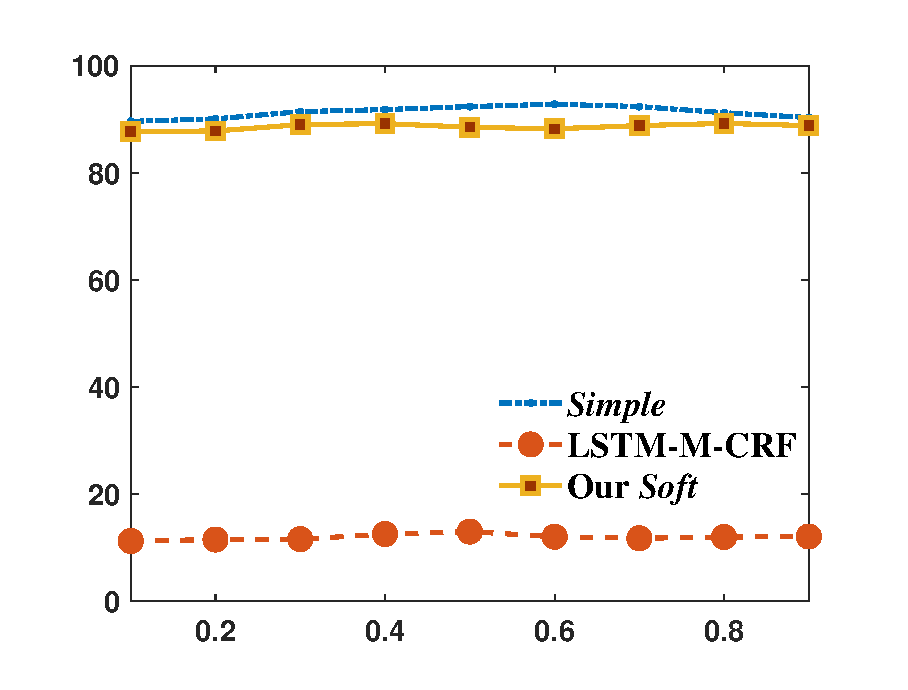
\includegraphics[width=2.4in]{Figures/conll2003precision.eps}
		%			\vspace{-5mm}
		\caption{Precision}
	\end{subfigure}
	\begin{subfigure}{0.45\linewidth}
		\centering
		\includegraphics[width=2.4in]{Figures/conll2003recall.eps}
		%			\vspace{-5mm}
		\caption{Recall}
	\end{subfigure}
	\begin{subfigure}{0.45\linewidth}
		\centering
		\includegraphics[width=2.4in]{Figures/conll2003.eps}
		%			\vspace{-5mm}
		\caption{$F$-score}
	\end{subfigure}
	%	}
	\caption{Precision, Recall and $F$-score with different $\rho$ on CoNLL-2003 dataset. }
	%	\vspace{-2mm}
	\label{fig:diffp}
\end{figure*}


%	\paragraph{Convergence Analysis}
%%\subsection{Convergence Analysis}
%We study the convergence of the $q$ distribution by evaluating the performance after each iterative training iteration. 
%Figure \ref{fig:cv} (left) shows the precision, recall and $F$-score performance of our {\it soft} variant on CoNLL-2003 dataset. 
%We can see the $F$-score keeps increasing and fluctuates at around 90 when the number of iteration is more than 3. 
%As expected, our approach performs similarly to the {\it Simple} baseline where the precision is high but recall is low. 
%The iterative process significantly improve the recall as well as the overall $F$-score until the $q$ distribution gradually converges. 
%In a sense, the iterative training process can retrieve many of the correct labels in training data. 
%
%
%With this definition, we can further calculate the recovery rate of correct labels in the training set recovered from the {\it soft} approach by counting the recovered labels. 
%
%\begin{figure}[t!]
%	\centering
%	\begin{subfigure}{0.5\columnwidth}
%		\centering
%		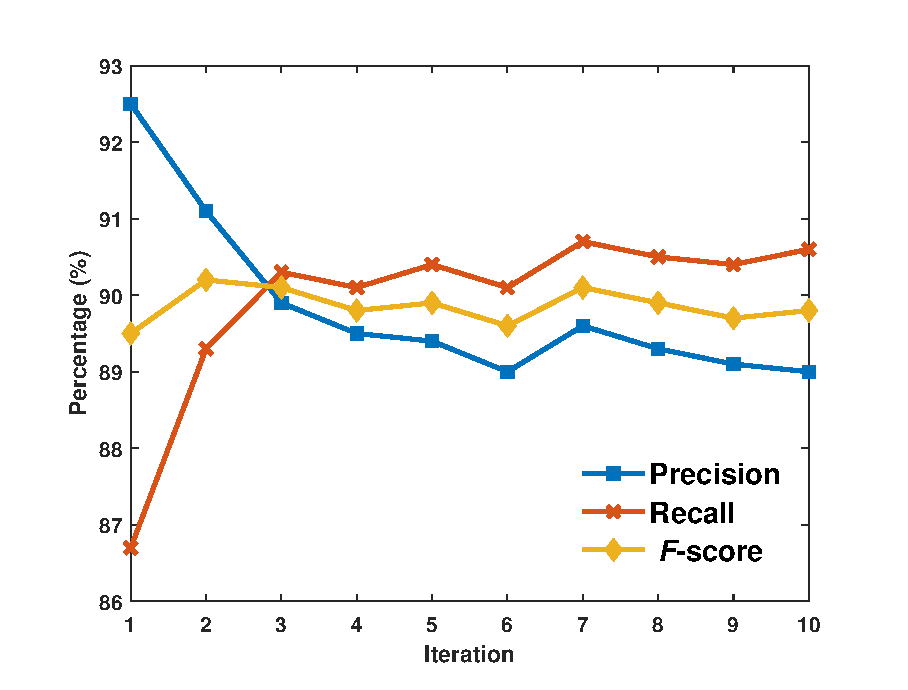
\includegraphics[width=1.4in]{imgs/cvperformance.eps}
%	\end{subfigure}
%	\begin{subfigure}{0.45\columnwidth}
%		\centering
%		\includegraphics[width=1.4in]{imgs/conll2003recover.eps}
%	\end{subfigure}
%	\caption{Precision, recall and $F$-score performance (left) on CoNLL-2003 development set and the recovery rate (right) after each iteration.}
%	\label{fig:cv}
%\end{figure} 
%The expectation can be calculated efficiently using the forward-backward algorithm. 
%Figure \ref{fig:cv} (right) shows the recovery rate of the training set generated from our approaches. 
%The recovery rate is consistent with the finding of the convergence in $F$-score where it becomes stable at around 94\% after the $3^{rd}$ iteration. 
%The fast convergence of our approach is consistent with the observation by \citet{nivre2008integrating} where they did not observe significant improvement after the first few iterations. 

%	\begin{table}[t!]
%		\centering
%		\scalebox{0.7}{
%		\begin{tabular}{lcccc}
%			\toprule
%			& CoNLL-2003 & CoNLL-2002 & Taobao & Youku \\\midrule
%			\textsc{Err} (\%) & {\color{white}0}3.13 &{\color{white}0}7.79 & 11.06& {\color{white}0}7.00 \\
%%			 ~~{\small\it --is annotation err} & 29.81 &42.86 &72.17 &  60.67\\
%			\bottomrule
%		\end{tabular}
%		}
%		\caption{Percentage of errors {\color{red}(at entity level)??} that are made by our approaches  {\color{red}(soft??)} but are corrected by the {\it Complete} model.}
%		\label{tab:unavailable}
%	\end{table}

%	\paragraph{Effect of Unavailable Labels}
%	{\color{red}We further conduct analysis on how the unavailable labels keep the  model away from achieving high performance.
%	Table \ref{tab:unavailable} shows the error ratio of entities that are incorrectly predicted by our {\it soft} variant but correctly predicted by the {\it Complete} model. 
%	Our approach obtains small error rate against the {\it Complete} model on all datasets except Taobao. 
%	We found that there are many entities in the test set of Taobao appear in the training set and many of them are not annotated in our experiments. }


\section{Dependency-based Solution: As a Future Work}

Essentially, the problem mentioned above is the missing annotations of \textsc{o} labels (\textit{i.e.,} false negative). 
Observing the relationships between the named entities and dependency trees, we can somehow infer that some dependency relations also have strong correlations with the \textsc{o} labels.
On the other hand, if some candidate spans are not forming subtrees, it is very likely that the span is not an entity.

Using such relationships, we present a dependency-based solution which can efficiently solve the incomplete annotation problem rather than iterative training. 
The underlying solution is a future work for solving this problem.


\subsection{Entity Candidate Selection}
Given the properties we observed in Chapter \ref{Chapter3} and Chapter \ref{Chapter4}, we identify some entity candidates and non-entity words before actual training. 
Specifically, we can perform the following pre-processing and then train a marginal CRF~\cite{greenberg2018marginal} but in a semi-Markov manner. 
\begin{itemize}
	\item Obtain the dependency parse trees with existing dependency parser.
	\item As entities are very likely to form subtrees, for those spans that cannot form subtree, we eliminate those spans in a semi-Markov model. 
	\item On the other hand, we also focus on the dependency relations. If some word are associated with dependency relations (e.g., \textit{neg}) are not possible to be entities, we also eliminate them to be non-entity words.
\end{itemize}

After the elimination process is done, we have a constrained space of named entities. 
We can train the model by maximizing  the marginalized log-likelihood.


\section{Conclusions}
In this work, we identified several limitations associated with previous assumptions when performing sequence labeling with incomplete annotations, and focused on the named entity recognition task.
%	In this work, we identify several limitations associated with previous assumptions when performing NER with incomplete annotations.
We present a novel and easy-to-implement solution that works under a realistic and challenging assumption on the incomplete annotations.
Through extensive experiments and analysis, we demonstrate the effectiveness of our approach. 
Finally, we present a potential dependency-based solution as a future work. 

Although we focused on the task of named entity recognition in this work, we believe the proposed approach may find applications in some other  sequence labeling tasks or other more general structured prediction problems where the issue of incomplete annotations is involved.



% under this challenging assumption. 
%	On the other hand, we would like to apply our approach on multiple datasets from different domains as the underlying scenario is more common in practice. 

%	In the future, we would like to apply our approach to datasets from different domains as the underlying scenario is more common in practice. 
%In the future, we would like to apply our approach on multiple datasets from different domains as the underlying scenario is more common in practice. 

